\documentclass[12pt]{article}
% add some essential packages, some might not be used

\usepackage[T1]{fontenc}
\usepackage[utf8]{inputenc}
\usepackage[usenames,dvipsnames]{color}
\usepackage{natbib}
\usepackage{authblk}
\usepackage{ragged2e}
\usepackage{amsmath}
\usepackage[a4paper,margin=1in,bottom=1.0in]{geometry}
\usepackage{url}
\usepackage{array}
\usepackage{bbding}
\usepackage{amssymb}
\usepackage{graphicx}  % mini page function
\usepackage{adjustbox}
\usepackage{subcaption}
\usepackage{booktabs}
\usepackage{float}
\usepackage{appendix} % appendix package
\usepackage{hyperref}
\usepackage{url}
\usepackage[english]{babel}
\usepackage{adjustbox}
\usepackage{enumitem}
\usepackage{textgreek}
\usepackage{bibentry}
\nobibliography*
\usepackage{lipsum}


\usepackage{listings}
\usepackage{wasysym}
\usepackage{amsthm}
\usepackage{framed}
\usepackage{bm}
\usepackage{booktabs}  % package for table line
% \usepackage{amsrefs?}  % ams citation style package


\usepackage{rotating} % for the horizontal page table

\usepackage{tikz}
\usetikzlibrary{calc}
\usetikzlibrary{matrix}
\usetikzlibrary{positioning}
\usepackage{color}
\usepackage{setspace}
\usepackage{xcolor}

\usepackage{tcolorbox} % package for making colorful box

 \setlength{\parskip}{0.15cm} % change the paragraph spacing
\renewcommand\labelitemi{$\vcenter{\hbox{\tiny$\bullet$}}$} % set the bullet size as tiny

% \newcommand*\rot{\rotatebox{90}} % for rotate text

\usepackage{sectsty} %package for section size

\sectionfont{\fontsize{14}{12}\selectfont} % Change the section font size

\subsectionfont{\fontsize{13}{12}\selectfont}
\subsubsectionfont{\fontsize{12}{12}\selectfont}

\newcommand\numberthis{\addtocounter{equation}{1}\tag{\theequation}} % new command



\theoremstyle{definition}
\newtheorem{definition}[subsection]{Definition}
\newtheorem{axiom}[subsection]{Axiom}
\newtheorem{example}[subsubsection]{Example}
\newtheorem{theorem}[subsection]{Theorem}
\newtheorem{proposition}[subsection]{Proposition}
\newtheorem{lemma}[subsection]{Lemma}


\usepackage{courier}

% tikzsetting

\usetikzlibrary{shapes,decorations,arrows,calc,arrows.meta,fit,positioning}

\tikzset{
    -Latex,auto,node distance =1 cm and 1 cm,semithick,
    state/.style ={ellipse, draw, minimum width = 0.7 cm},
    point/.style = {circle, draw, inner sep=0.04cm,fill,node contents={}},
    bidirected/.style={Latex-Latex,dashed},
    el/.style = {inner sep=2pt, align=left, sloped}
}

\lstset{language=Python}

\definecolor{mygreen}{rgb}{0,0.6,0}
\definecolor{mygray}{RGB}{145, 153, 165}
\definecolor{mymauve}{rgb}{0.58,0,0.82}

\lstset{
  backgroundcolor=\color{white},   % choose the background color; you must add \usepackage{color} or \usepackage{xcolor}; should come as last argument
  basicstyle=\footnotesize,        % the size of the fonts that are used for the code
  breakatwhitespace=false,         % sets if automatic breaks should only happen at whitespace
  breaklines=true,                 % sets automatic line breaking
  captionpos=b,                    % sets the caption-position to bottom
  commentstyle=\color{gray},    % comment style
  deletekeywords={...},            % if you want to delete keywords from the given language
  escapeinside={\%*}{*)},          % if you want to add LaTeX within your code
  extendedchars=true,              % lets you use non-ASCII characters; for 8-bits encodings only, does not work with UTF-8
  frame=single,	                   % adds a frame around the code
  keepspaces=true,                 % keeps spaces in text, useful for keeping indentation of code (possibly needs columns=flexible)
  keywordstyle=\color{RoyalBlue},       % keyword style
  language=Python,                 % the language of the code
  morekeywords={*,...},            % if you want to add more keywords to the set
  numbers=left,                    % where to put the line-numbers; possible values are (none, left, right)
  numbersep=5pt,                   % how far the line-numbers are from the code
  numberstyle=\tiny\color{gray}, % the style that is used for the line-numbers
  rulecolor=\color{black},         % if not set, the frame-color may be changed on line-breaks within not-black text (e.g. comments (green here))
  showspaces=false,                % show spaces everywhere adding particular underscores; it overrides 'showstringspaces'
  showstringspaces=false,          % underline spaces within strings only
  showtabs=false,                  % show tabs within strings adding particular underscores
  stepnumber=2,                    % the step between two line-numbers. If it's 1, each line will be numbered
  stringstyle=\color{mymauve},     % string literal style
  tabsize=2,	                   % sets default tabsize to 2 spaces
  title=\lstname                   % show the filename of files included with \lstinputlisting; also try caption instead of title
}

\numberwithin{equation}{section}
\numberwithin{figure}{section}
\numberwithin{table}{section}


% Define colors
\definecolor{cmd}{HTML}{F7F7F9}
\DeclareMathOperator{\di}{d\!}

\newcommand{\pr}{$\mathbb{P}$}
\newcommand{\pre}{\mathbb{P}}

\begin{document}

\title{Machine Learning Project: machine learning part}
\author{Michael}
\date{}
\maketitle



\section{Features Construction}

As it has been discussed in the last section, the task can be formatted as the standard classification problem, which regards the kinship as one class and the nonkinship as other. The binary classification on the kinship in the dataset can only be implemented when the dimensions of features are less than the number of observations. Since we have 3598 pairs of kinship in the dataset, the features constructed from the dataset has to be less than 3598. Without employing too much computing power, the feature for each picture is constructed as follows:
\begin{itemize}
	\item Step 1: for picture $p_i = [224, 224, 3]$, take the first two dimensions and let the transformed picture $x_i = [224, 224]$;
	\item Step 2: let $w = x_ix_i^T$, and then take the eigenvalues of $w$, and let $f_i = \texttt{eigenvalues(w)}$;
	\item Step 3: for each pair of kinship, calculate the element-wise differences of features: $$d_p = f_{p1} - f_{p2}$$
	\item Step 4: among all pictures, randomly match the new pairs and make sure those pairs are not kinship, then calculate the element-wise differences of features by repeating step 1 to 3. 
\end{itemize}


\section{Properties of Features}

With 3598 pairs of kinships and 3598 pairs of nonkinships, we can examine the properties of features before using machine learning models to do classification. Figure 2.1 presents the comparison of features for kinship and nonkinship. 
\begin{figure}[H]
  \centering
  \begin{subfigure}[b]{0.49\textwidth}
    \centering
    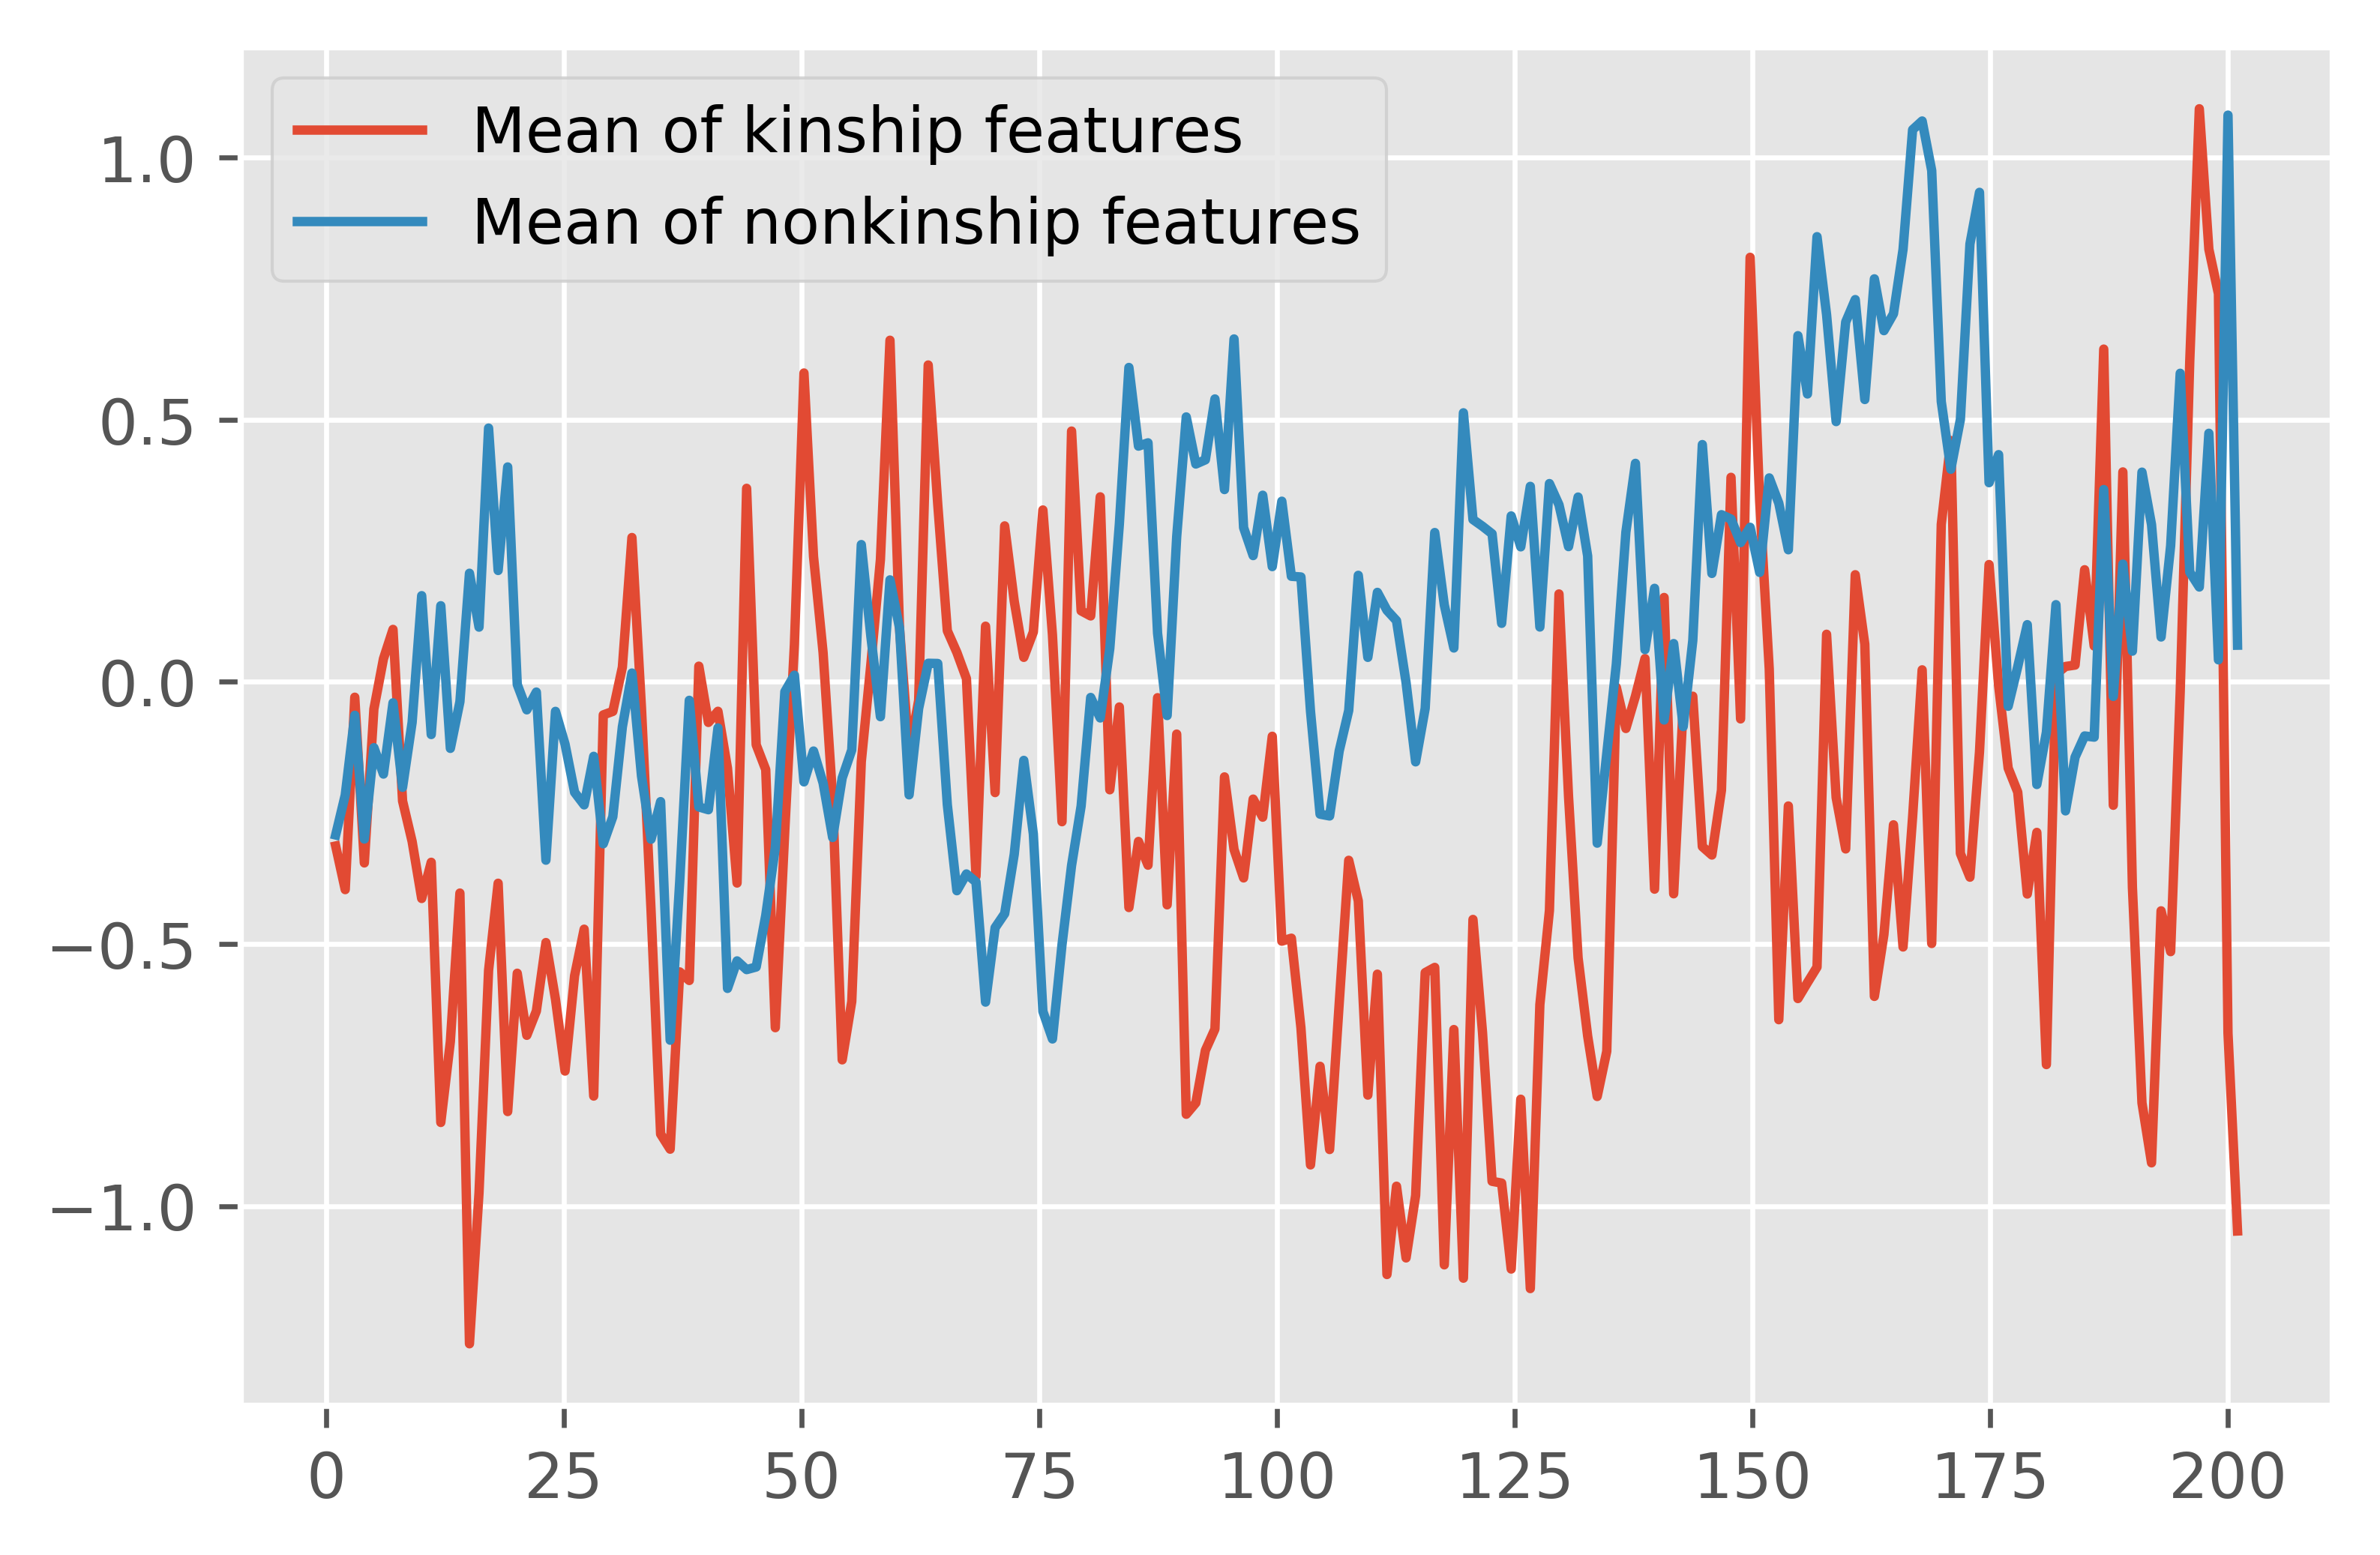
\includegraphics[width=\textwidth]{meanfeatures}
  \end{subfigure}
  \begin{subfigure}[b]{0.49\textwidth}
    \centering
    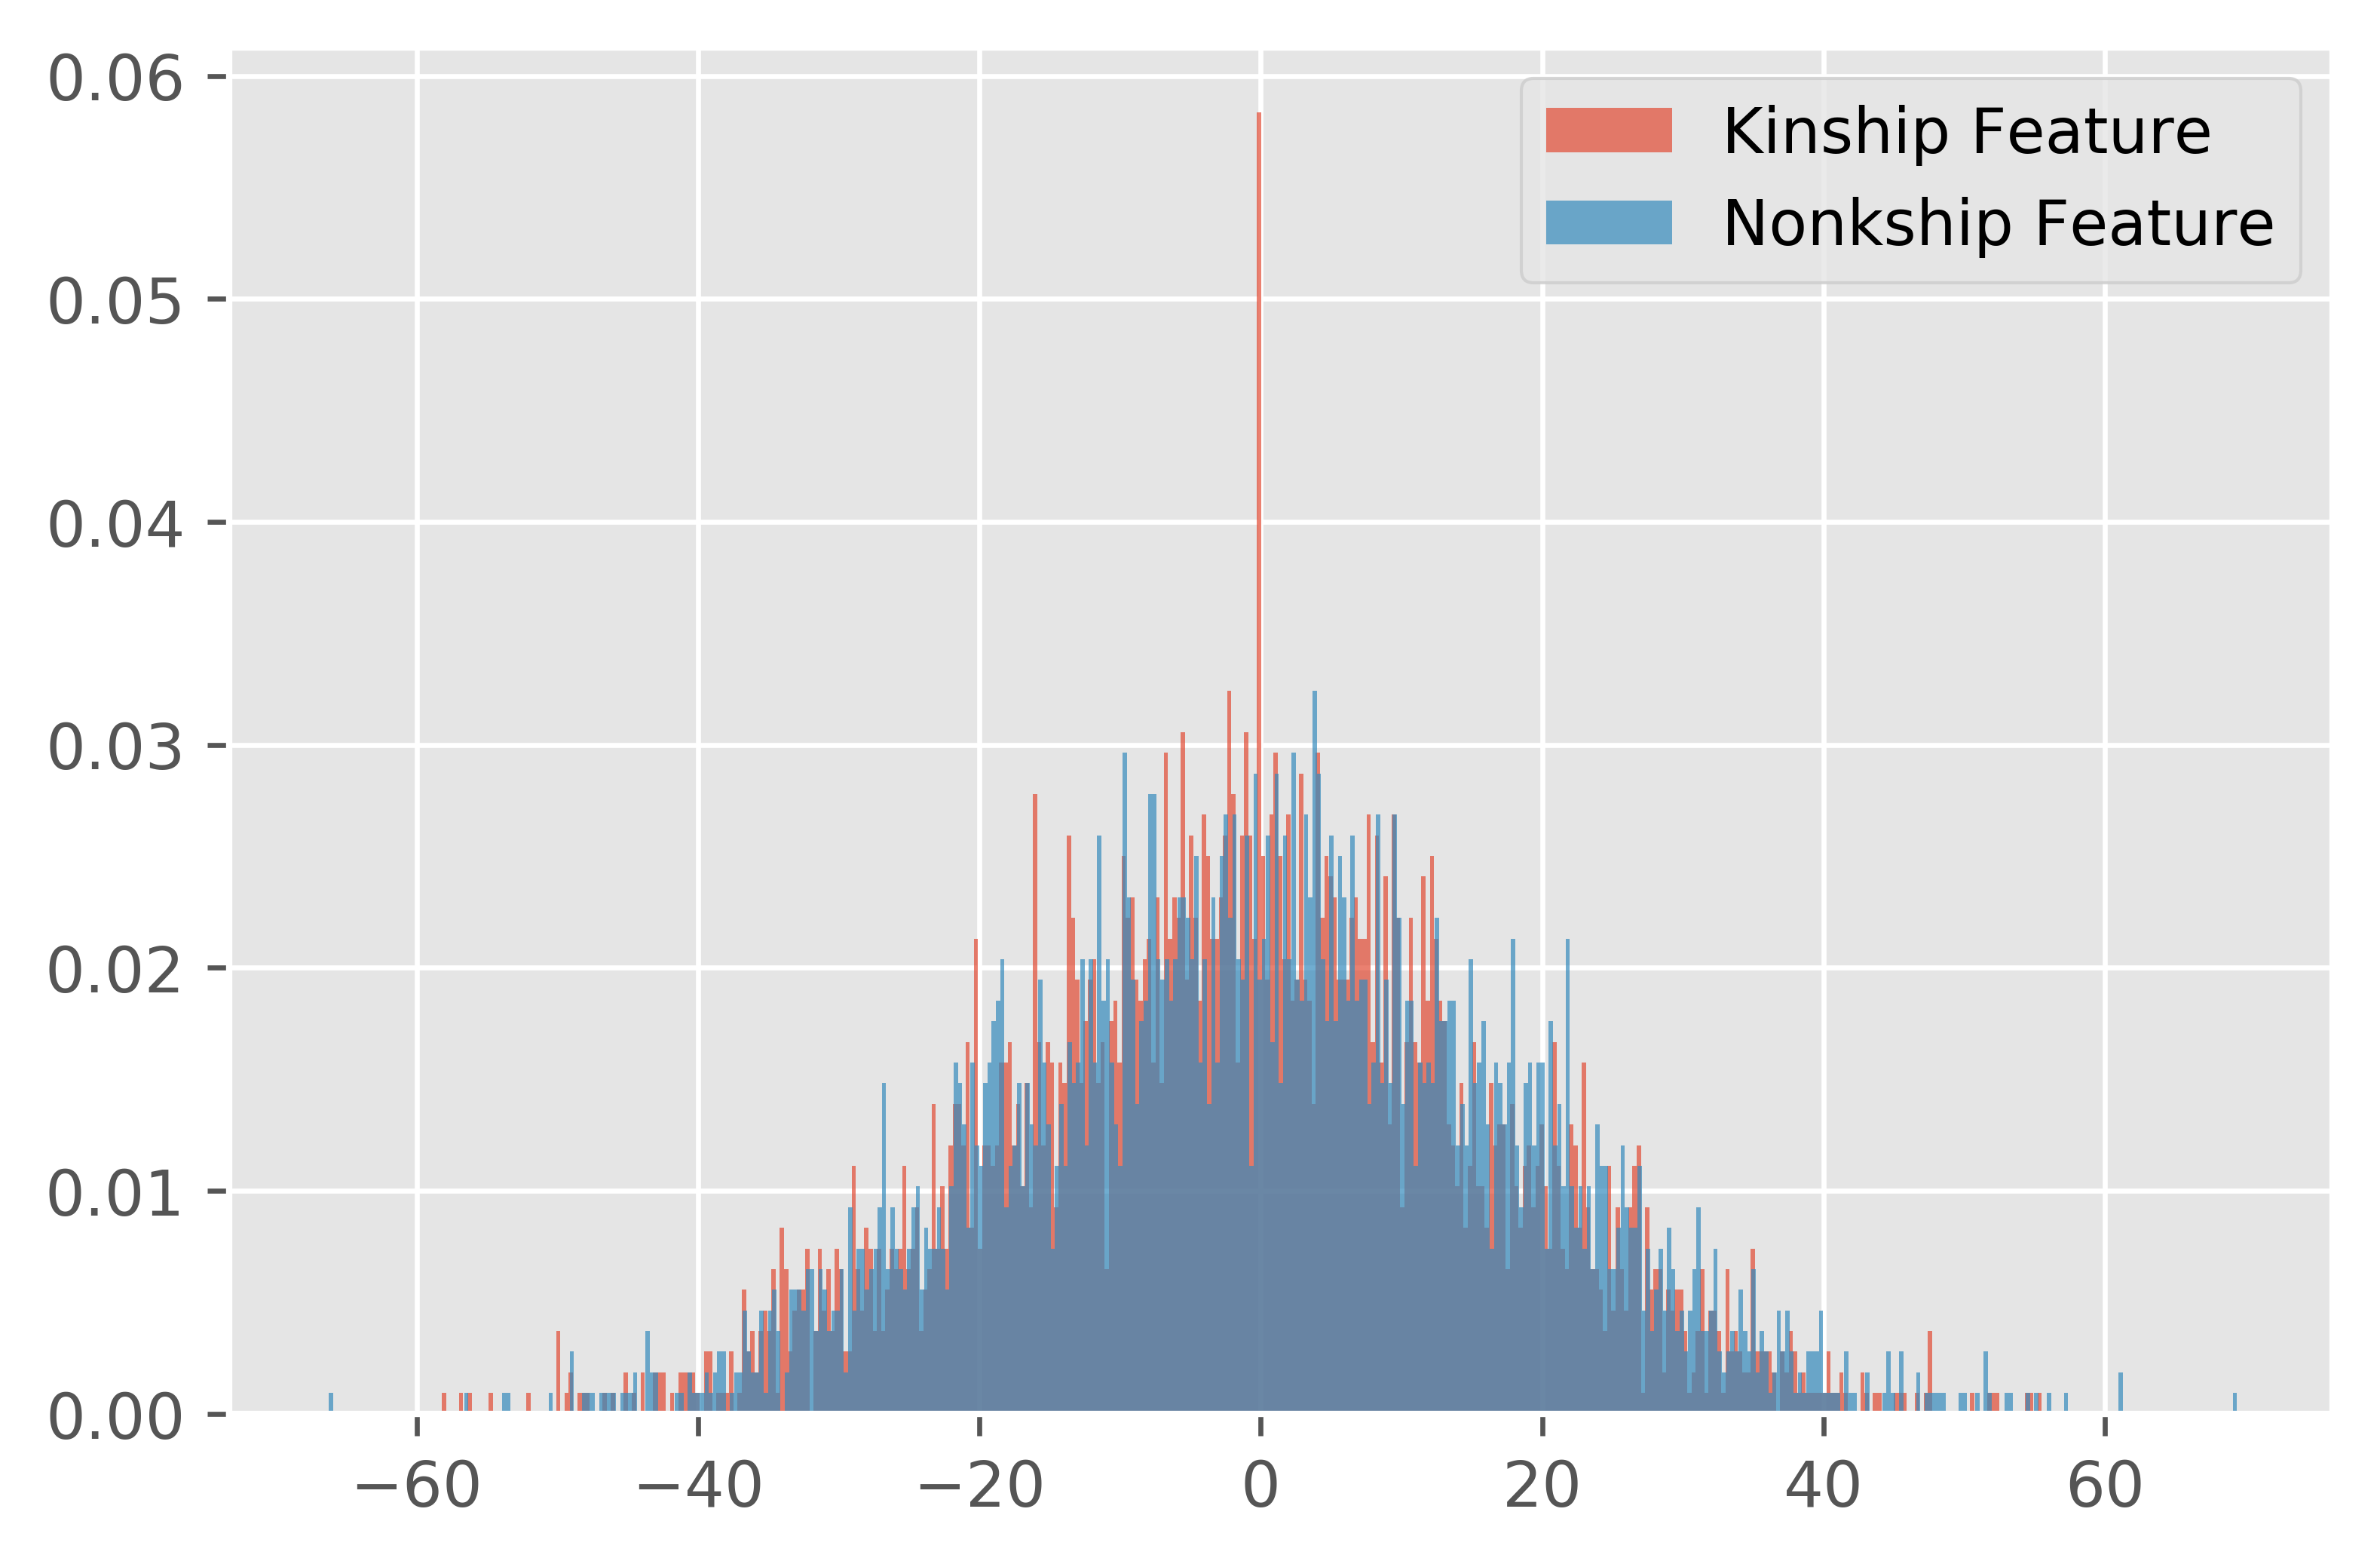
\includegraphics[width=\textwidth]{histfeatures}
  \end{subfigure}
  \caption{Comparison of Kinship and Nonkinship}
\end{figure}
According to Figure 2.1, certain amount of feature differences exist between kinship and nonkinship pairs. However, the difference is not big enough to allow the model to detect the boundaries for classification. What's more, the distributions of selected features for kinship and nonkinship are homogenous. This means that the models by using Gaussian densities will not work well on those features.

When it comes to the distances of features differences, figure 2.2 gives the comparison. Again, the distributions of the distances\footnote{The distance is measured by Euclidean distance.} are very similar to each other for kinship pairs and nonkinship pairs. This brings the challenges for the methods employing the distance measurements, such as KNN, etc.  
\begin{figure}[!htpb]
	\centering
	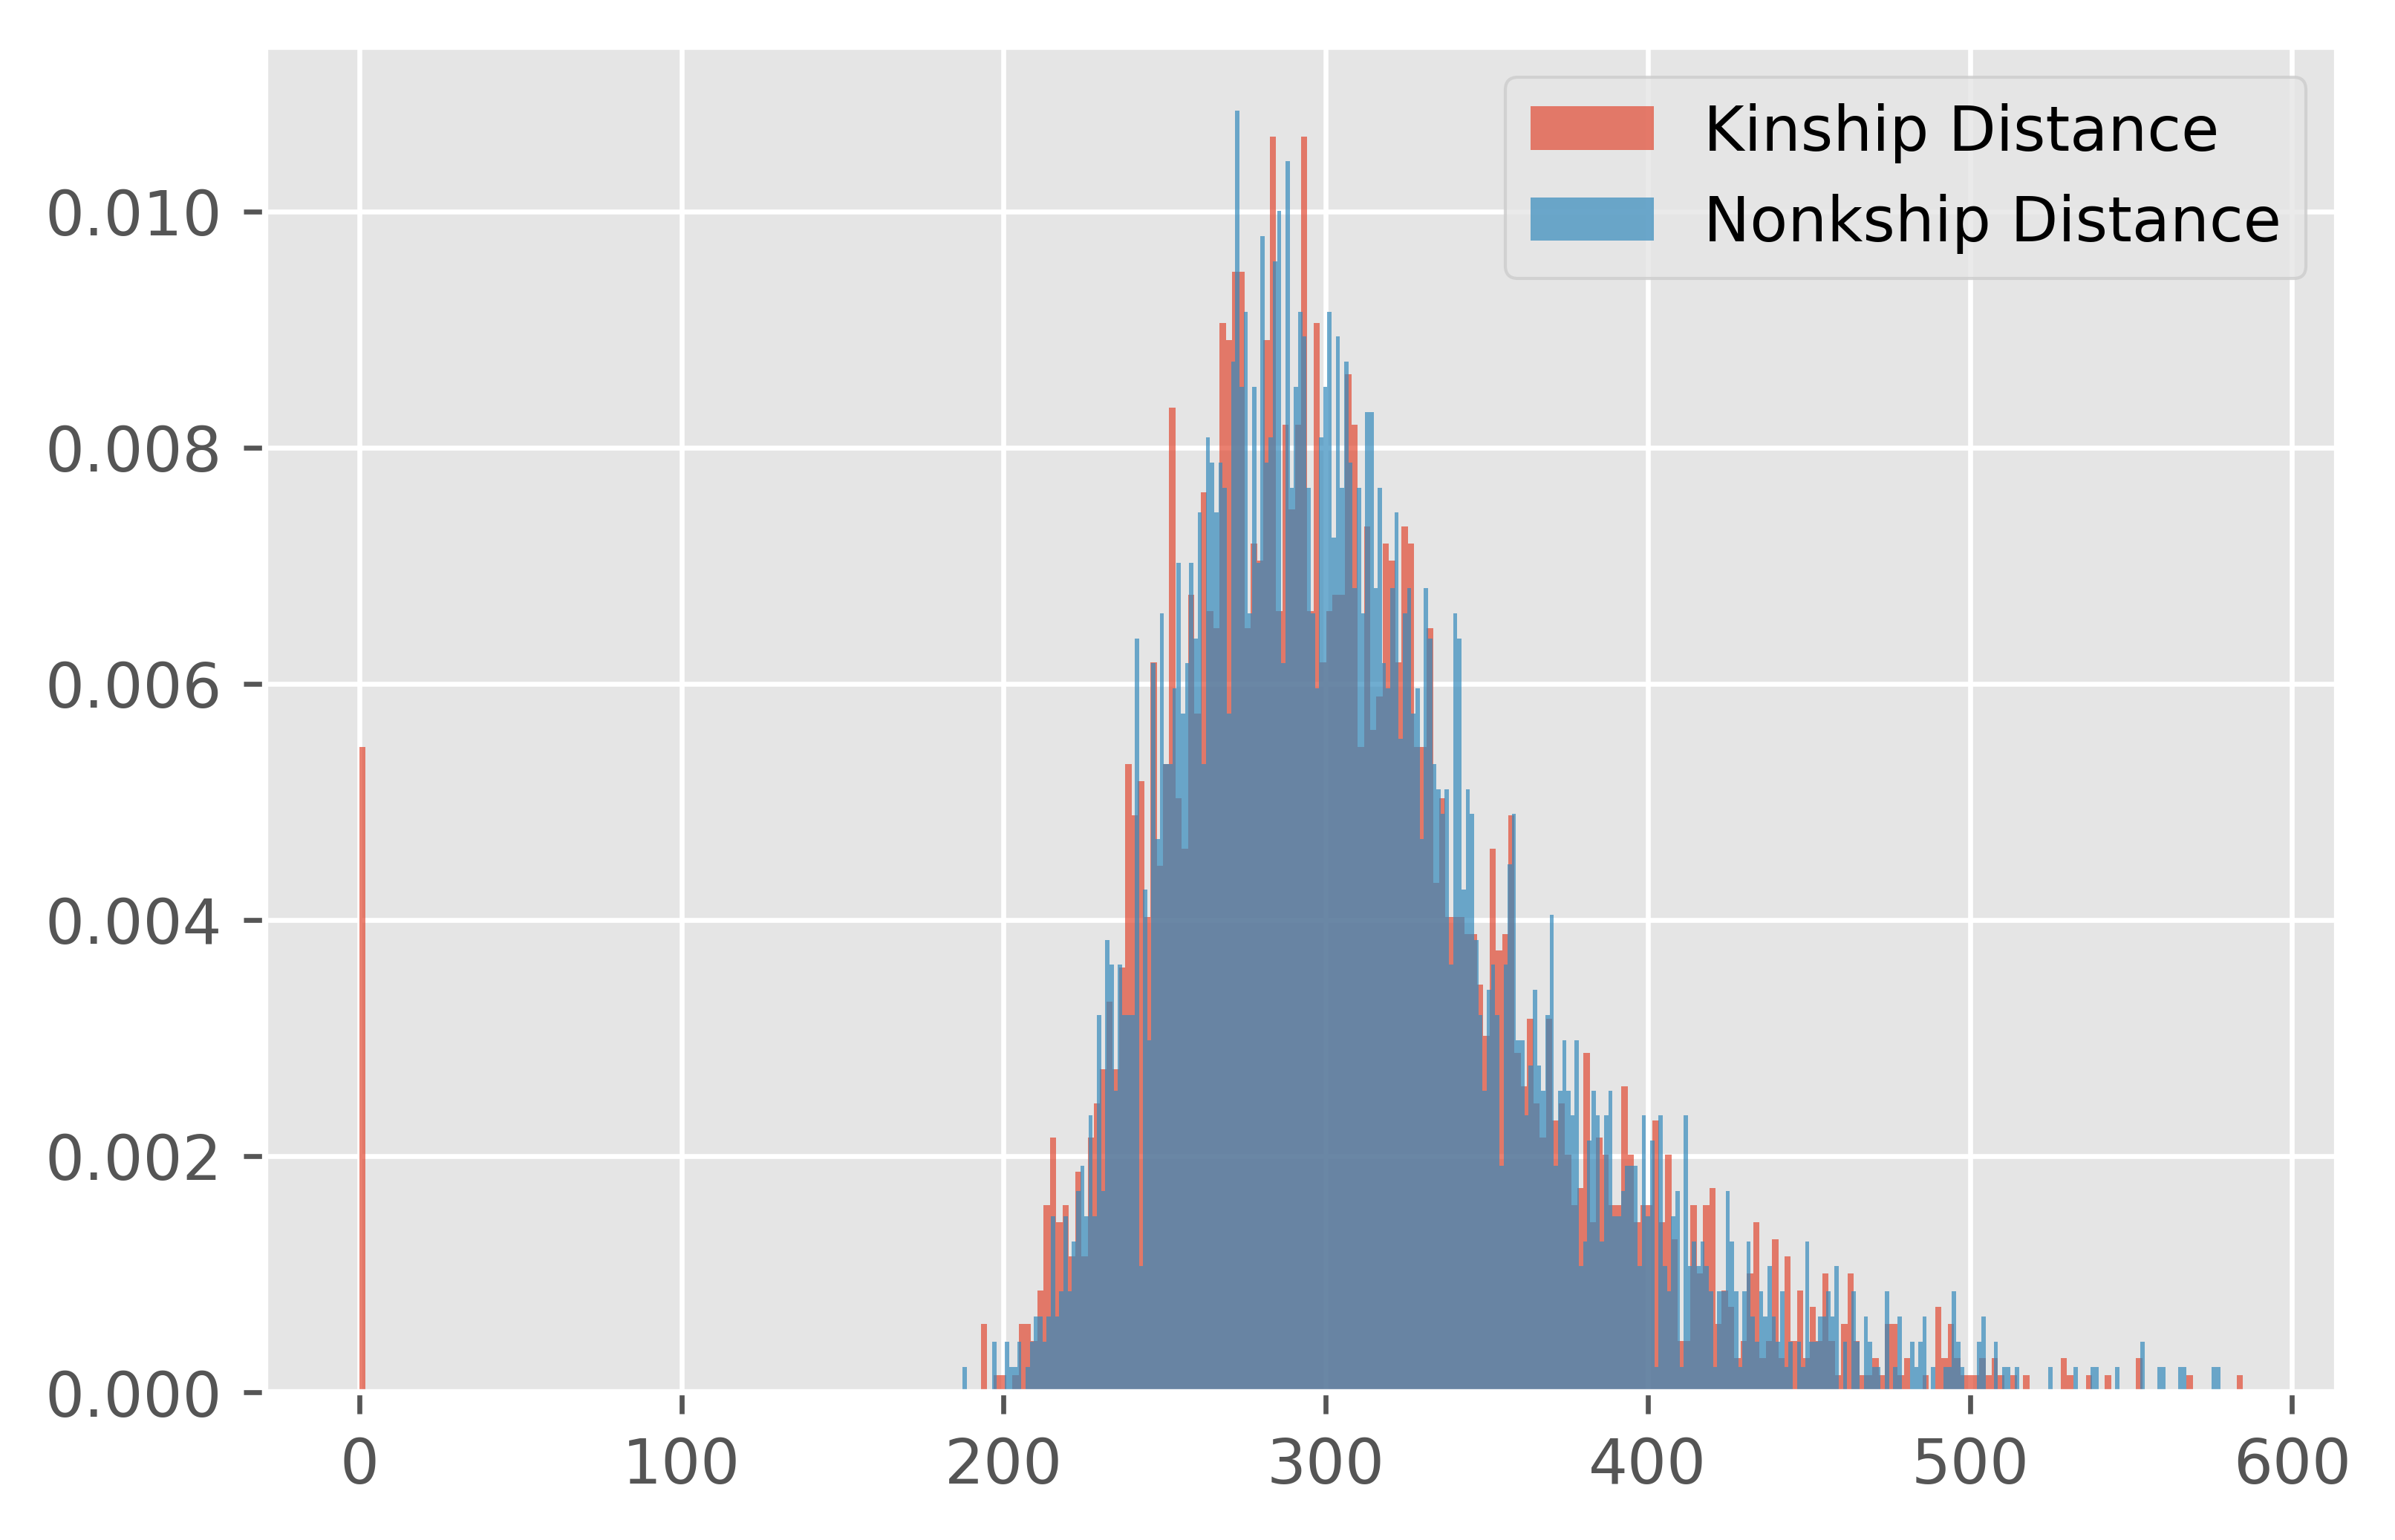
\includegraphics[width=0.8\textwidth]{histdistance}
	\caption{Histogram of Distances}
\end{figure}

\section{Review and Results of Machine Learning Models}

Before presenting the results, it is worth to review the main models in machine learning field. In our project, we have employed linear discriminant analysis (LDA), quadratic discriminant analysis (QDA), logistic regression, naive Bayes classification, k-nearest-neighbor classification (KNN), support vector machines (SVM) and neutral network methods. 

For LDA, QDA and logistic regression, they all employe the Gaussian densities. Suppose we model each class density as multivariate Gaussian 
\begin{align}
	f_k(x) = \frac{1}{(2\pi)^{p/2} | \Sigma_k|^{1/2}} \exp[-\frac{1}{2}(x - \mu_k)^T \Sigma_k^{-1}(x-\mu_k)],
\end{align}
where LDA assumes that the classes have a common covariance matrix $\Sigma_k = \Sigma \forall k$, and the observations are classified by using the following function
\begin{align}
	\delta_k(x) = x^T \Sigma^{-1} \mu_k - \frac{1}{2} \mu_k^T \Sigma^{-1} \mu_k + \log \pi_k	
\end{align}
However, QDA assumes that each class has its own covariance matrix $\Sigma_k$, and the observations are classified by using the following function
\begin{align}
	\delta_k(x) = -\frac{1}{2} \log |\Sigma_k| - \frac{1}{2} (x - \mu_k)^T \Sigma_k^{-1} (x - \mu_k) + \log \pi_k
\end{align}

The logistic regression uses the continuous function (or map) between covariates $x$ and dependent variable probability $\pi$:
\begin{align}
  \pi = h_{\theta}(x) = \frac{e^{\theta' x}}{ 1 + e^{\theta' x}} = \frac{1}{1+ e^{-\theta' x}}
\end{align}
where the general format
\begin{align*}
  g(z) = \frac{1}{1+e^{-z}}
\end{align*}
is called the logistic function. With this function, the log-likelihood function was employed to find the coefficients:
\begin{align*}
  L(\theta) & = \prod_{i=1}^m P(y^{i}| x^{i}; \theta) \\
  & = \prod_{i=1}^m (h_{\theta}(x))^y (1 - h_{\theta}(x))^{1-y}
\end{align*}

The naive Bayes classification has the same structure with LDA and QDA, which means it also assumes the certain density function behind the model. 

The k-nearest-neighbor methods employs the Euclidean distance in feature space:
\begin{align*}
	d_i = || x_i - x_0 ||, 
\end{align*}
where the distance is used to search for the nearest neighbors. The classification is made by following the majority rule. 

Table 3.1 gives the results from different machine learning methods. The comparison of those results can show why some methods outperform others. For instance, LDA wins out over the QDA as the classes in the dataset has the common covariance matrix. This means the QDA will not work well as it assumes the classes should have separate covariance matrixes.
\begin{table}[H]
	\centering
	\renewcommand{\arraystretch}{1.2}
	\caption{Results of Different ML Methods}
			\begin{tabular}{lcccl}
		\hline 
		\hline 
		Methods & Accuracy & True Positive & AUC  &  Explanations\\
		\hline 
		LDA &  $54.28\%$& $55.09\%$ & $54.28\%$& Common covariance 
\\
		\hline 
		QDA &  $51.69\%$ & $52.61\%$ & $51.68\%$&Separate covariance  \\
		& & & & for each class \\
		\hline 
		Logistic &  $54.47\%$ & $55.25\%$ &$54.46\%$ & Log Likelihood\\
		\hline 
		Bayes & $52.43\%$ & $62.97\%$ & $51.83\%$&Diagonal variance \\
		\hline 
		KNN & $53.41\%$ & $66.54\%$ &$52.39\%$ & Neighbors = 3 \\
		\hline 
		SVM & $56.55\%$ & $59.85\%$ & $56.49\%$ & scale the input\\
		\hline 
		Neural NW & $54.18\%$ & $65.08\%$ & $53.47\%$ & layer size = 12, 6\\
		\hline 
	\end{tabular} 
\end{table}










\newpage
\bibliography{/Users/Michael/Documents/MachineLearning/ML.bib}
\bibliographystyle{apalike}
\end{document}